\documentclass[10pt,preprint]{sigplanconf}
\usepackage{times}

\usepackage{datetime}
\usepackage{url}
\usepackage{hyperref}
\usepackage{graphicx}
\usepackage{afterpage}
\usepackage{minted}

\graphicspath{ {images/} }

\copyrightyear{2017} 


% No date in title area.
\date{}

\authorinfo{Greg Harper}


% Actual document begins below.
\begin{document}

\title{Delving into the Linux Kernel} 
\maketitle

\begin{abstract}

A recent trend in personal computing is a movement away from desktop computers and workstations and towards laptops and small personal devices such as tablets and cell phones. These devices are generally disconnected from wall power and running off of their batteries for long periods of time, lending more and more importance to a balance between performance and power efficiency. Simultaneously, embedded devices are becoming more and more powerful, up to the point where many now embedded versions of common operating systems, often Linux. The combination of these two trends has made power management a main focus in recent development of the Linux kernel. For the aforementioned devices to have reasonably performant CPUs while also being power efficient, it is necessary that the CPUs be able to power down when not in use. This leads to the CPUidle subsystem of the Linux kernel. The CPUidle subsystem comes into play when a CPU is idle (when it has no current task to execute). The subsystem then decides how much to power down the CPU, such that it will optimize power savings while still being able to resume operation as necessary to meet scheduling constraints. Various CPU architectures offer differing definitions of the low power states available to the CPUidle subsystem, and therefore CPUidle must define and support an interface which allows it to optimize for any given CPU, as well as containing the logic for the power optimization process. This report will discuss the architecture of the CPUidle subsystem, with emphasis on the control flow of the idle loop, the interaction(s) between the CPUidle subsystem and other subsystems of the Linux kernel, and the various interfaces and software constructs supported and defined by the CPUidle subsystem. In addition it will go into depth on the architecture of the structures which control the power optimization decisions, known as governors. Finally, it will discuss an interesting case of complexity that arises in the CPUidle subsystem when managing the idle states of coupled processors.

\end{abstract}

\section{CPUidle in the Context of the Linux Kernel}

\begin{figure}[h]
\caption{Map of Full Linux Kernel v4.1}
\centering
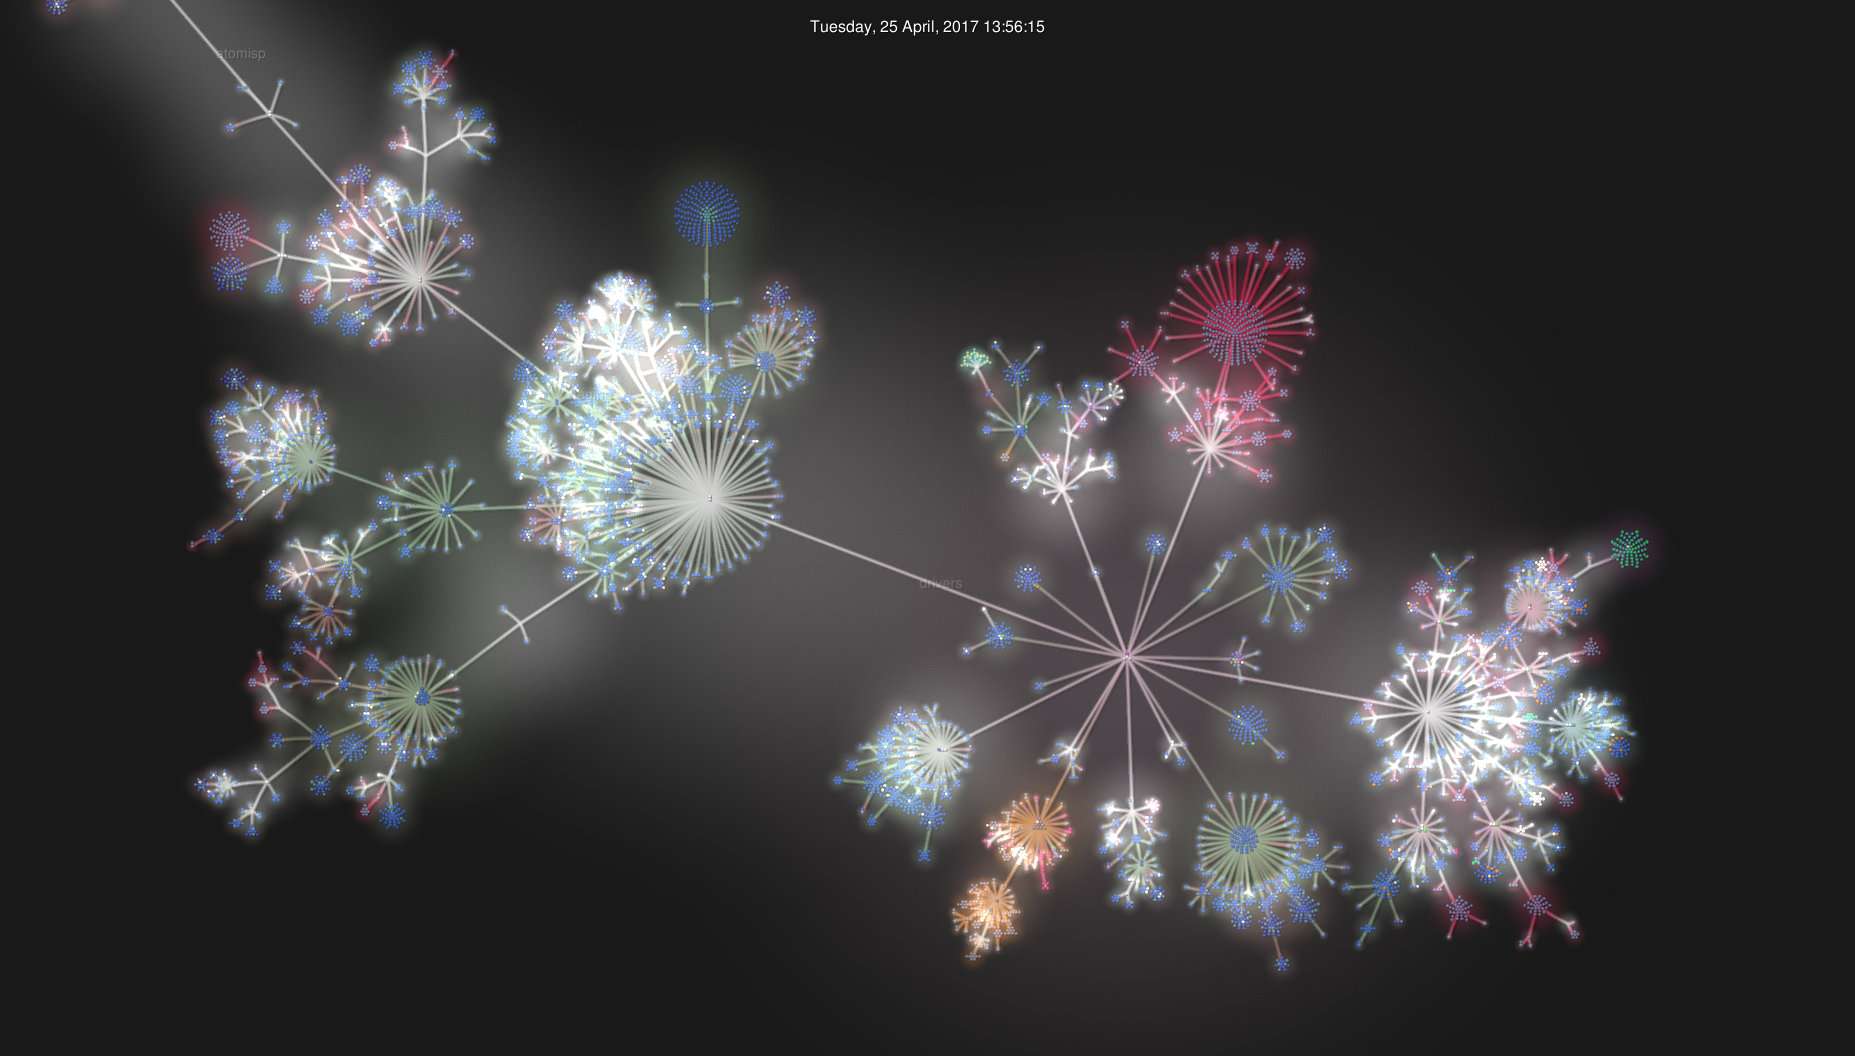
\includegraphics[width=\columnwidth]{full_kernel}
\end{figure}

The CPUidle subsystem is part of the power management architecture of the Linux kernel. It is responsible for ensuring that the system’s CPUs are always in the lowest power state possible. A large portion of time, there is nothing for a given CPU to do, especially in a multicore processor or a multiprocessor system. When a CPU has no task to execute, it is considered to be idle, and is in an idle loop. During this loop, the CPU is simply executing a “do nothing” instruction and waiting for further instructions. There is a lot of wasted power which goes into executing the idle loop while operating in a fully-on state. Therefore, modern CPUs have “c states,” where progressively deeper states equate to progressively lower power usage. As always in computer systems, there is generally a performance cost in exchange for power savings, and the cost of entering these c states tends to be a minimum exit latency for bringing the CPU back up into full operation. This latency means that performance and scheduling constraints limit the deepest state a CPU can be put into upon entering the idle loop, and it is the job of the CPUidle subsystem to calculate the deepest state the system's CPUs can enter at a given time, as well as controlling the interface for actually instructing the CPUs to enter said states. It is left up to the CPU drivers to supply the information needed by CPUidle to describe the c states, and to implement the software structures and behavior needed to control the physical hardware. 

\begin{figure}[h]
\caption{Kernel Source Code Pertaining to CPUidle Subsystem}
\centering
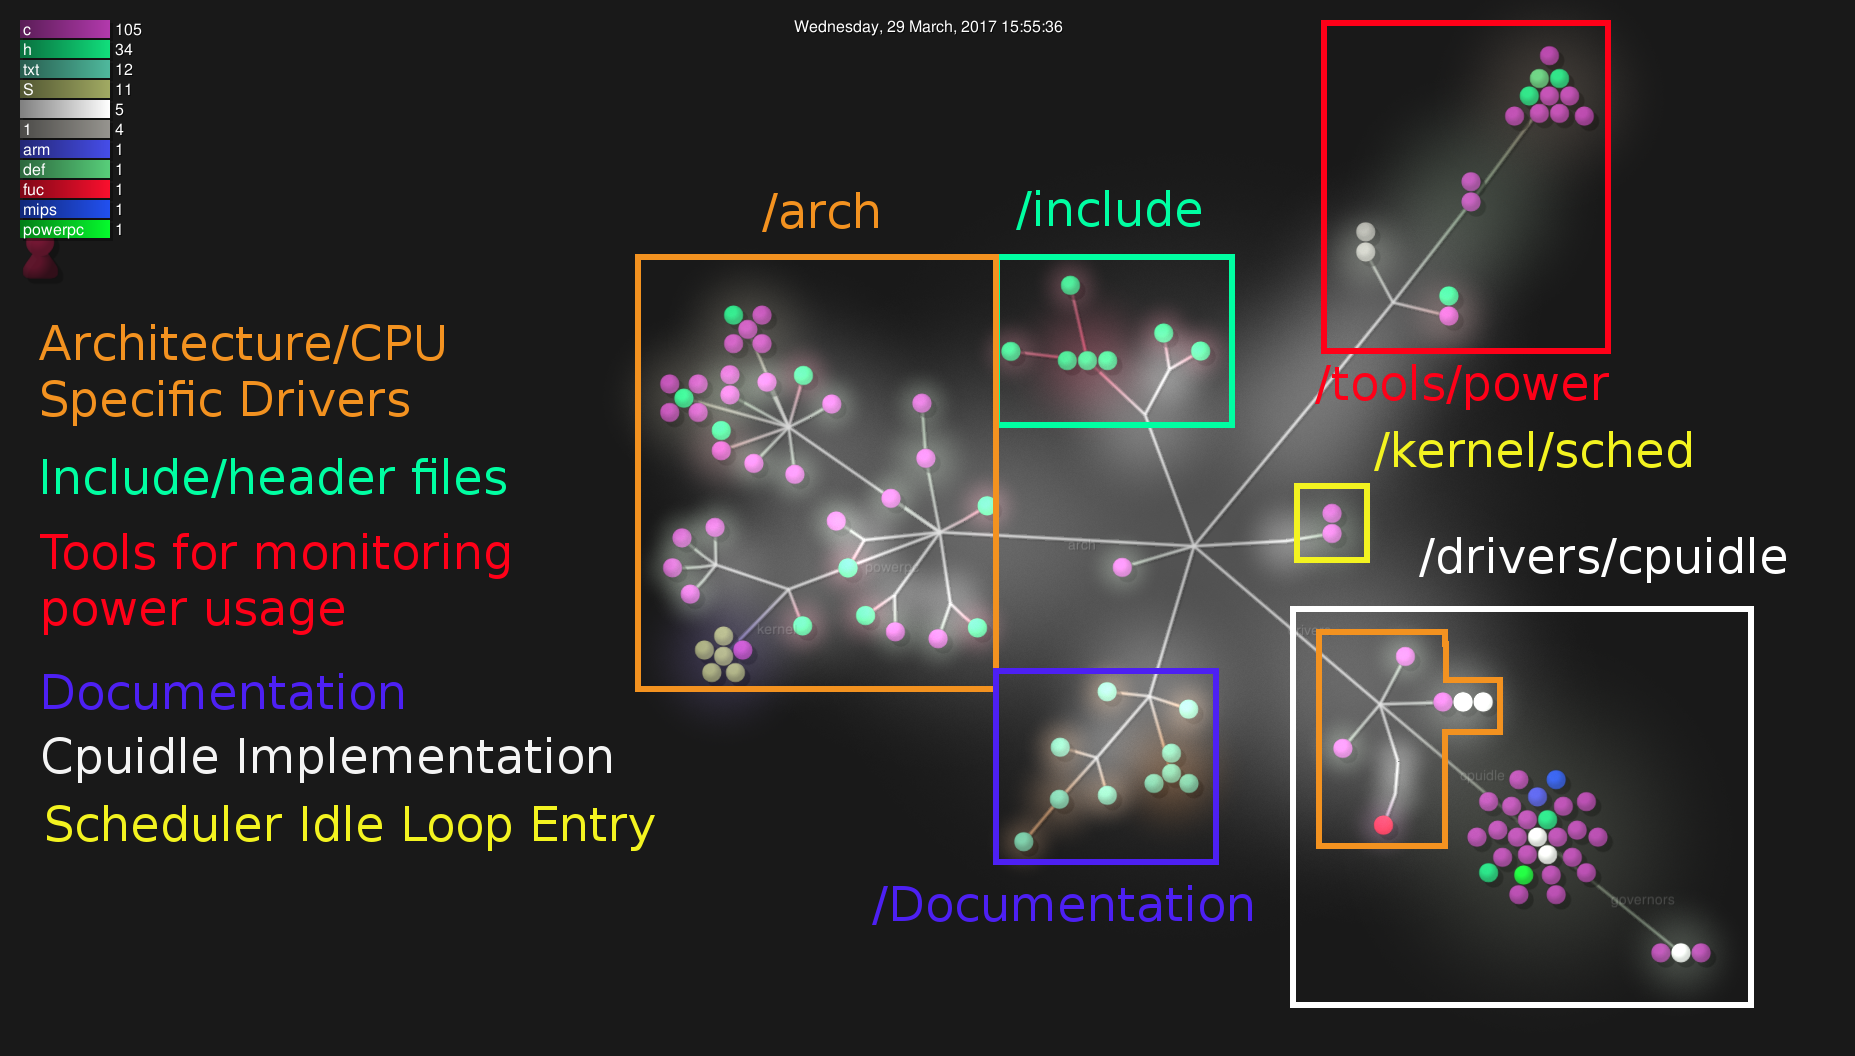
\includegraphics[width=\columnwidth]{cpuidle_files_web_annotated}
\label{fig:ann}
\end{figure}

As can be seen in figure \ref{fig:ann}, there are six primary regions in the kernel source code pertaining to the CPUidle subsystem. The documentation is self-explanatory, and the include and header files are primarily interface definitions of the CPUidle interfaces for different hardware architectures. The real meat of CPUidle is in the other four regions. The central implementation of the subsystem is in the \textbf{drivers/CPUidle} folder. In this folder is where the primary logic is defined for choosing c states and communicating with the drivers when to change to a different power state. This logic is accessed by the scheduling subsystem when it schedules the idle loop, from the files \textbf{idle.c} and \textbf{idle\_task.c} in the scheduler directory. The CPU drivers and other architecture specific CPUidle drivers are in the \textbf{/arch} directory, with a small scattering in the \textbf{/drivers} directory. Finally, several tools for measuring and reporting the power management and performance of the CPUidle subsystem are in the tools section of the source code. Though all aspects of these 4 areas hold the potential to be interesting, for the sake of constraining the scope of this report, focus will be on the control flow of the idle process and the architecture and implementation of the general CPUidle subsystem, rather than the architecture specific implementations of idle states or the implementation of performance and efficiency measuring tools.

   \subsection{The Idle Process and CPUidle Inter-Subsystem Interactions}
   The beginning of the CPUidle sub-system's job doesn't actually occur within the CPUidle code, but rather the scheduler. Whenever the Linux kernel is up and running, the idle process is continuously rescheduled, usually with the lowest priority. This process, defined in \textbf{/kernel/sched/idle\_task.c}, is duplicated once for each CPU, and throws an error if it is ever moved from the CPU it is initially assigned to. In this manner, each CPU contains an idle process, which only runs if there is nothing else for that CPU to do. When it comes time for a CPU to run it’s idle task, the scheduler begins execution of the flow shown in detail in figure \ref{fig:detail}. However, a basic version of the subsystem level control flow is depicted in figure \ref{fig:simple}.
   
    \begin{figure}[h]
    \caption{Simplified CPUidle Subsystem Level Control Flow}
    \centering
    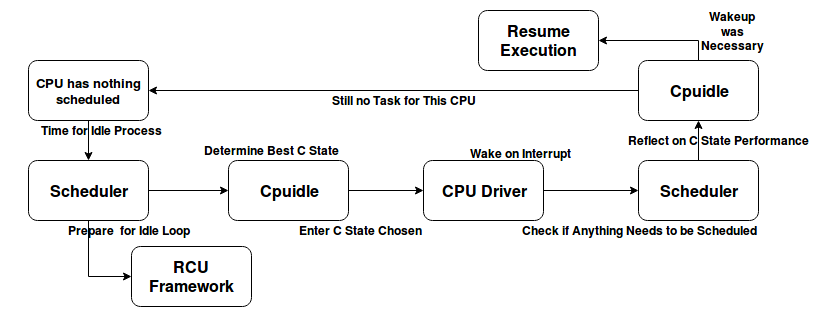
\includegraphics[width=\columnwidth]{Idle_Flow_Simple}
    \label{fig:simple}
    \end{figure}
    
    The CPUidle subsystem interacts primarily with the scheduler and the drivers for the CPU that is entering the idle state. Though it is not clear from the above diagram, the sheer number of different supported architectures means that in terms of raw lines of code, the most interaction is definitely in the drivers. However, each driver must uphold the interface supported by the CPUidle architecture, so these interactions are all the same from the perspective of the CPUidle subsystem. In addition, the RCU framework, a subsystem which helps keep memory consistent during simultaneous read-write operations must be told when a CPU is going idle, and when it wakes up. This communication is also handled by the CPUidle subsystem. Though not shown in the above figure, CPUidle also interacts with the interrupt subsystem as enabling and disabling various interrupts is necessary for maintaining idle states for the correct amount of time.  Finally, measurement of c state effectiveness and governor performance is handled by the pm\_qos subsystem, a subsystem in the power management framework.
    A much more detailed control flow is depicted in the figure \ref{fig:detail}. External subsystems are treated as black boxes in this diagram, as they are not within the scope of this report. In addition, the CPUidle governors are also black-boxed, as the implementation will be discussed later in this report
    \afterpage{

    \begin{figure}[p]
    \caption{Full Control Flow of CPUidle idle Process}
    \centering
    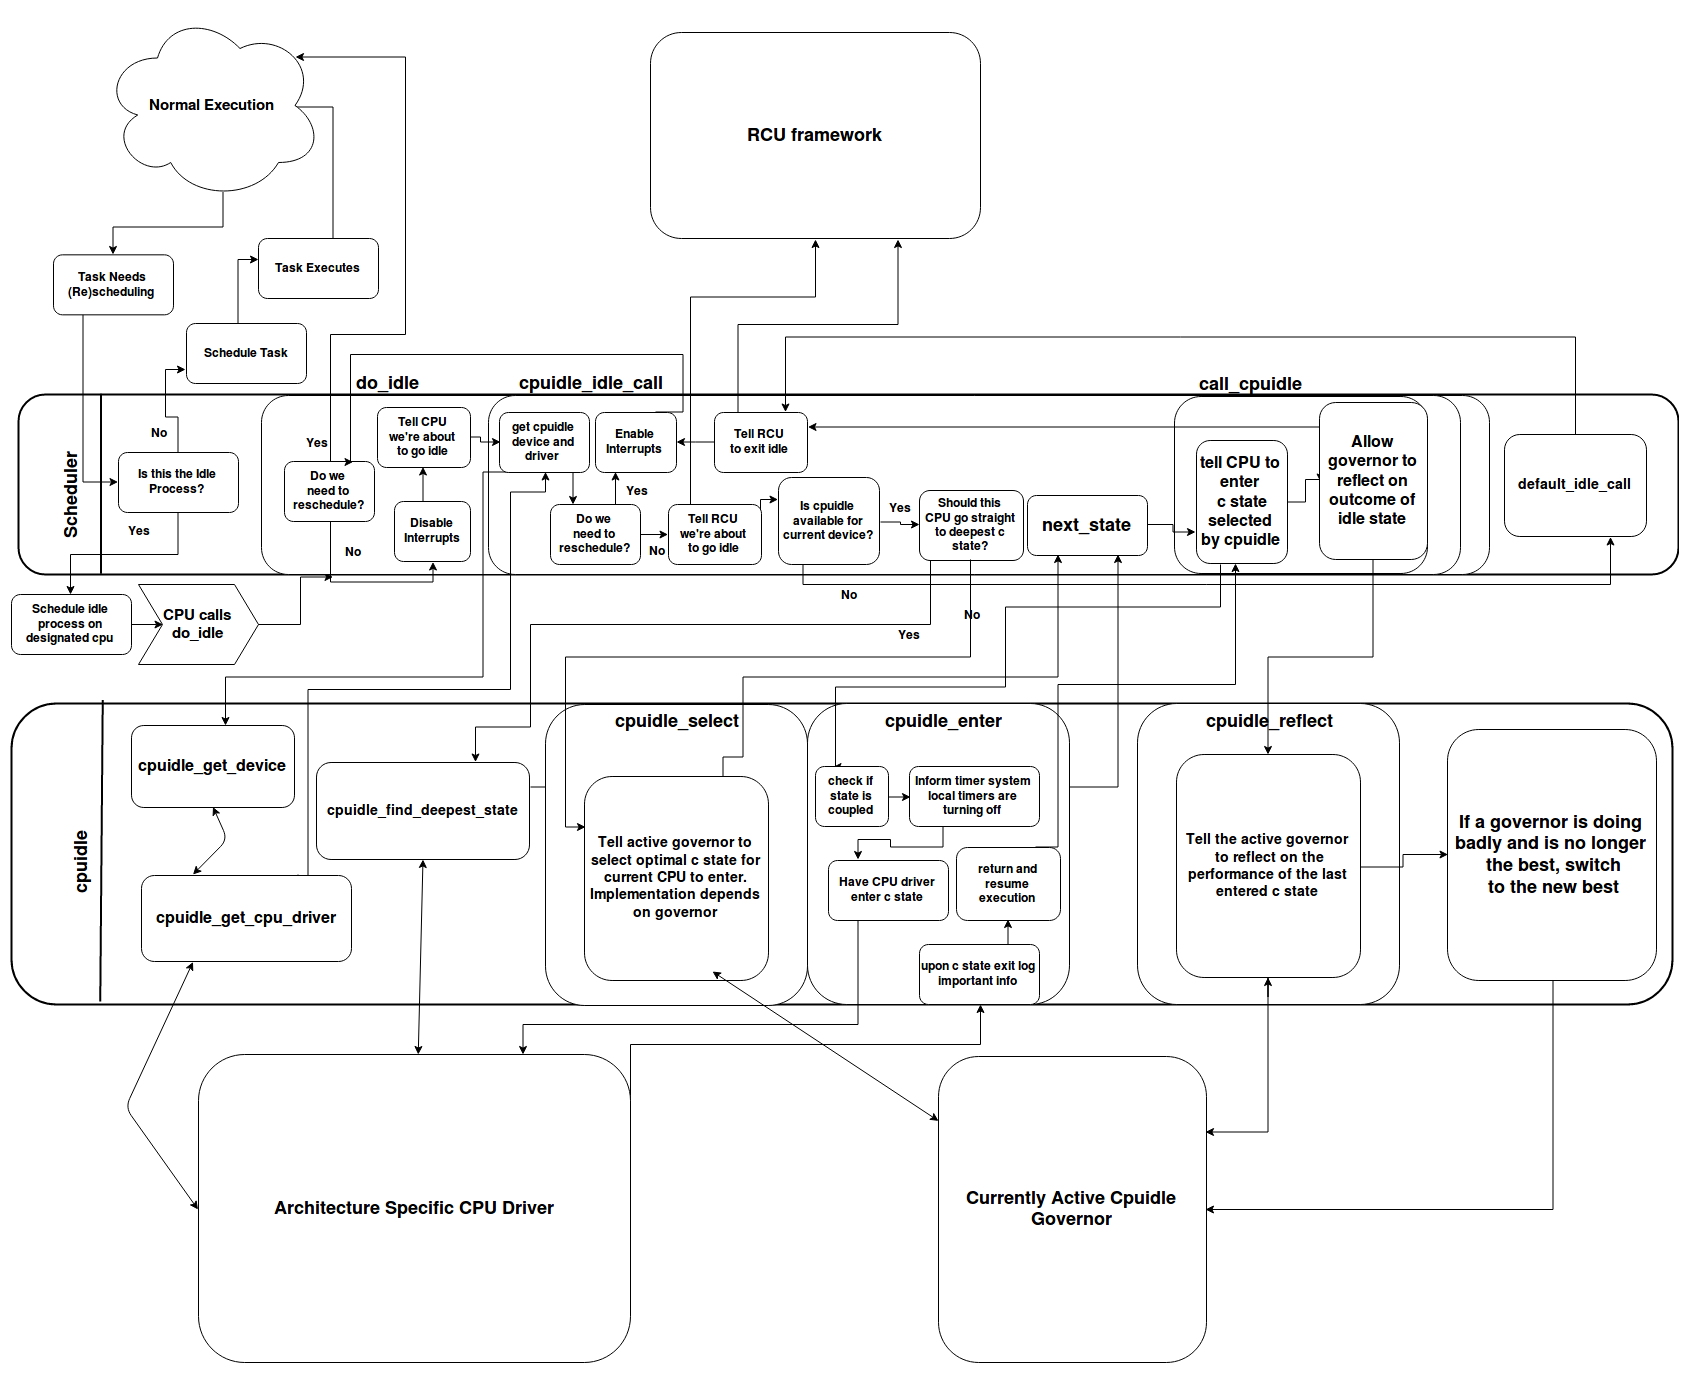
\includegraphics[width=\textwidth]{Idle_Loop}
    \label{fig:detail}
    \end{figure}
    
    \clearpage
    }
    \afterpage{
    \subsection{The Interfaces of the CPUidle Subsystem}
    
    Though the idle loop is where the main control flow of the CPUidle subsystem actually occurs, the interfaces of the subsystem are what allow the magic to happen behind the scenes. In addition, these interfaces are crucial for concealing the individual CPUidle CPU device drivers from the rest of the kernel. Because these interfaces are in place, the rest of the kernel can pretend that all CPU architectures provide the same CPUidle implementation, and can interact only with the generic CPUidle subsystem. For developer purposes, there is also a \textbf{sysfs} interface for interacting with the CPUidle subsystem from user space. And finally, there is the governors interface, which will be discussed in depth later in this report.
    \begin{figure}[h]
    \caption{The Interfaces of the CPUidle Subsystem\newline Image taken from (1)}
    \centering
    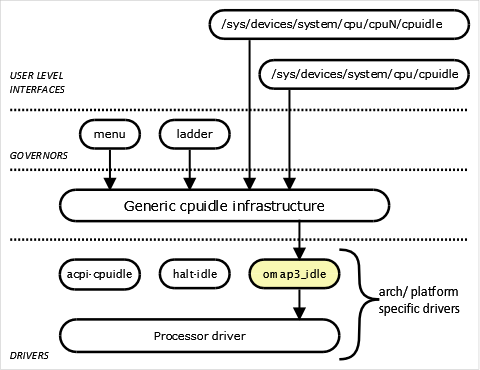
\includegraphics[width=\columnwidth]{Cpuidle}
    \label{fig:interfaces}
    \end{figure}
    
            
              
    }
    \clearpage
    
  \subsubsection{The CPUidle State Interface}
  
    
\begin{minted}
[
frame=lines,
framesep=2mm,
baselinestretch=1.2,
fontsize=\footnotesize,
linenos
]
{C}

struct CPUidle_state {
      char            name[CPUIDLE_NAME_LEN];
      char            desc[CPUIDLE_DESC_LEN];

      unsigned int    flags;
      unsigned int    exit_latency; /* in US */
      int             power_usage; /* in mW */
      unsigned int    target_residency; /* in US */
      bool            disabled; /* disabled on all CPUs */

      int (*enter)    (struct CPUidle_device *dev,
                      struct CPUidle_driver *drv,
                      int index);
//...
};

\end{minted}

The CPUidle\_state interface represents a c state for a processor. It contains the information a  CPUidle governor needs to decide whether to enter the state, and a function pointer to the entry point of the state.

\subsubsection{The CPUidle Device Interface}

\begin{minted}
[
frame=lines,
framesep=2mm,
baselinestretch=1.2,
fontsize=\footnotesize,
linenos
]
{C}

struct CPUidle_device_kobj;
struct CPUidle_state_kobj;
 struct CPUidle_driver_kobj;

struct CPUidle_device {
        unsigned int            registered:1;
        unsigned int            enabled:1;
        unsigned int            use_deepest_state:1;
        unsigned int            cpu;

        int                     last_residency;
        struct CPUidle_state_usage      states_usage[CPUIDLE_STATE_MAX];
        struct CPUidle_state_kobj *kobjs[CPUIDLE_STATE_MAX];
        struct CPUidle_driver_kobj *kobj_driver;
        struct CPUidle_device_kobj *kobj_dev;
//...
};


\end{minted}

The device interface is metadata that links the CPU hardware driver with the CPUidle subsystem. It contains flags about how the “owned” CPU is allowed to enter c states, and  about which CPU it corresponds to, as well as the usage information for all the c states supported by the given CPU. It also wraps the kobjects that implement the driver, the CPUidle device for this CPU, and an array of kobjects representing all the available states for this CPU.
\clearpage

\subsubsection{The CPUidle Driver Interface}

\begin{minted}
[
frame=lines,
framesep=2mm,
baselinestretch=1.2,
fontsize=\footnotesize,
linenos
]
{C}

struct CPUidle_driver {
        const char              *name;
        struct module           *owner;
        int                     refcnt;
//...
        /* states array must be ordered in decreasing power consumption */
        struct CPUidle_state    states[CPUIDLE_STATE_MAX];
        int                     state_count;
        int                     safe_state_index;
//...
extern void disable_CPUidle(void);
extern bool CPUidle_not_available(struct CPUidle_driver *drv,
                                  struct CPUidle_device *dev);

extern int CPUidle_select(struct CPUidle_driver *drv,
                          struct CPUidle_device *dev);
extern int CPUidle_enter(struct CPUidle_driver *drv,
                         struct CPUidle_device *dev, int index);
extern void CPUidle_reflect(struct CPUidle_device *dev, int index);
//...
extern struct CPUidle_driver *CPUidle_get_driver(void);

extern int CPUidle_enable_device(struct CPUidle_device *dev);
extern void CPUidle_disable_device(struct CPUidle_device *dev);

extern struct CPUidle_driver *CPUidle_get_cpu_driver(struct CPUidle_device *dev);
extern int CPUidle_find_deepest_state(struct CPUidle_driver *drv,

extern void CPUidle_use_deepest_state(bool enable);

\end{minted}


The CPUidle Driver interface is simultaneously the most straightforward and the most important. It simply contains the metadata necessary to connect it with its kobject owner (the actual implementation of the driver for the given CPU architecture). However, it is also where all the interface functions for the CPUidle system are exposed. The most important of these are the primary interface points accessed by the idle process during the idle loop.


\textbf{CPUidle\_select} instructs the CPU to ask the active governor which state to enter.

\textbf{CPUidle\_enter} instructs the given CPU driver to have the idle CPU enter the given c state.

\textbf{CPUidle\_reflect} instructs the active governor to reflect upon the correctness of entering the state which was just left.

\subsubsection{The CPUidle Sysfs Interface}


There are several user space interfaces available for interacting with the CPUidle subsystem, accessible at the file path \textbf{/sys/devices/system/cpu/CPUidle}

By default, there are two read only interfaces revealing the current driver being used: 

\textbf{/sys/devices/system/cpu/CPUidle/current\_driver}

and the current governor being used: 

\textbf{/sys/devices/system/cpu/CPUidle/current\_governor\_ro}

\vfill
\clearpage
However, if the boot option \textbf{idle\_sysfs\_switch} is enabled, there is also a read only list of available governors: 

\textbf{/sys/devices/system/cpu/CPUidle/available\_governors}

and a read-write interface allowing the user to get and set the current governor:

\textbf{/sys/devices/system/cpu/CPUidle/current\_governor}

In addition, there is information about each CPU’s c states available through another sysfs interface:

\textbf{/sys/devices/system/cpu/cpuX/CPUidle/}

and

\textbf{/sys/devices/system/cpu/cpuX/CPUidle/stateY}

In these cases X is the number of the CPU of interest and Y is the number of the state of interest. This interface is read only, and if the state information is read, the following information is displayed: \newline
 \textbf{desc} : Small description about the idle state (string)\newline
 \textbf{disable} : Option to disable this idle state (bool)\newline
 \textbf{latency} : Latency to exit out of this idle state (in microseconds)\newline
 \textbf{name} : Name of the idle state (string)\newline
 \textbf{power} : Power consumed while in this idle state (in milliwatts)\newline
 \textbf{time} : Total time spent in this idle state (in microseconds)\newline
 \textbf{usage} : Number of times this state was entered (count)\newline

\subsubsection{The CPUidle Governor Interface}

\begin{minted}
[
frame=lines,
framesep=2mm,
baselinestretch=1.2,
fontsize=\footnotesize,
linenos
]
{C}

struct CPUidle_governor {
    char                    name[CPUIDLE_NAME_LEN];
    struct list_head        governor_list;
    unsigned int            rating;

    int  (*enable)          (struct CPUidle_driver *drv,
                                    struct CPUidle_device *dev);
    void (*disable)         (struct CPUidle_driver *drv,
                                    struct CPUidle_device *dev);

    int  (*select)          (struct CPUidle_driver *drv,
                                    struct CPUidle_device *dev);
    void (*reflect)         (struct CPUidle_device *dev, int index);
};


\end{minted}

The final interface of CPUidle is perhaps the most important. The CPUidle governor is the structure which performs the central duty of the CPUidle subsystem, choosing which idle state to enter for the optimal power/performance tradeoff. The governor interface is deceptively simple, only requiring a field for the governor’s rating, and 4 crucial function pointers. Enable and disable are straightforward, but select and reflect are where the power of the governor lies. Select uses the governor’s internal logic to select the next c state for the given CPU, while reflect updates the governor’s rating based on the performance on the last c state chosen. This enables the kernel to select the optimal governor for choosing c states, and to update which governor is being used on the fly.

\section{Ladder and Menu: CPUidle Governors}

Many governors can be operational within the CPUidle subsystem at once, and the subsystem will simply select the best one to make the decision about which c states should be used in the idle loop. This is done using the rating field of the governors, where a higher rating denotes a better governor. When a given governor is active, every time the CPU exits an idle state the CPUidle subsystem calls the reflect method of the active governor, and the governor adjusts its rating based on the performance of the c state it chose. If the governor has been making bad decisions, its rating will drop and it will eventually be replaced by a different governor. As of version 4.1, the linux kernel contains two different governors, the ladder governor and the menu governor.

\clearpage

\subsection{The Ladder Governor}

The ladder governor is the original governor created alongside the current architecture of the CPUidle subsystem. The ladder governor is a simple governor which constantly moves deeper into the hierarchy of c states until a failed state is reached, at which point it backs up one step. It is possible for the ladder governor to pick a much shallower c state than it previously did, if the known latency requirements of the system suggest that this is necessary to meet scheduling constraints. However, it is not possible for the ladder governor to move more than 1 level deeper in the c state hierarchy, which means that it is almost always not fully optimizing the power efficiency of the CPU. Also, if a given c state is disabled for any reason, then all states deeper than that state are also considered disabled for the purposes of the ladder governor. This means that disabling a c state when the ladder governor is active can have serious drawbacks for the power efficiency of a system.

\subsection{The Menu Governor}

The menu governor is a more recent addition to the kernel compared to the ladder governor. It was developed based on the observation that almost all system events requiring a CPU to wake from an idle state were either periodic and predictable timer events or IO interrupts. As timer events are practically fully predictable, this suggests that the only unknown factors affecting the lowest possible c state for a CPU are IO events. The menu governor attempts to predict the duration that will occur from when it is told to select an idle state for a processor and the next IO event for that processor, and use this information to pick a truly optimal c state. Unlike the ladder governor, the menu governor always has free reign to pick any enabled c state. This means that it can make large jumps deeper into the c state hierarchy, possibly drastically increasing the power efficiency of the system when compared to the ladder governor. However, this carries the risk that the menu governor will make a bad prediction, and will cause performance issues due to excessive latency while a CPU is exiting from the idle process.

\subsection{Which Governor is Better?}

Asking which governor is better is somewhat of a trick question, as both are better in different cases. When the kernel is compiled with a constant CPU timer tick, the ladder governor tends to be better, as a frequent timer interrupt waking the processor from an idle state wreaks havoc with the interrupt prediction of the menu governor. However, if a compile or boot time option is selected to disable this tick during the idle process, then the menu governor typically leaps ahead, as its ability to make educated guesses and large leaps in terms of c state depth lead to much more optimal power savings. This is not unnoticed by the kernel developers: if the option is selected to enable the CPU tick even during the idle loop, then the ladder governor is given a much higher initial rating than the menu governor.


\begin{minted}
[
frame=lines,
framesep=2mm,
baselinestretch=1.2,
fontsize=\footnotesize,
linenos
]
{C}

static int __init init_ladder(void)
{
        /*
         * When NO_HZ is disabled, or when booting with 
         * nohz=off, the ladder governor is better so 
         * give it a higher rating than the menu governor.
         */
    if (!tick_nohz_enabled)
            ladder_governor.rating = 25;
    return cpuidle_register_governor(&ladder_governor);
}
\end{minted}

\section{Dealing with the Complexity of Coupled CPUs}

A final note about the CPUidle subsystem is the solution developed in order to deal with the complexity added to a multicore or multiprocessor system when some of the CPUs in the system are coupled. Two or more CPUs are considered coupled when for any reason, they must always reside in the same c state. Some examples of application processors with coupled cores are the Nvidia Tegra 2 and the TI OMAP4460. The Tegra 2 has coupled cores by design; the CPU cores must be powered down in a specific order, with CPU0 being the last core to enter a low power state. The OMAP4460, on the other hand, has coupled cores because of a hardware bug. In order to work around this defect, while one core is powering up the other core must run a workaround to make sure the system reached the correct state.

When a cluster of CPUs is coupled for any reason, a specific process must be run to bring them into a low power state. First, all of the CPUs must be brought into a state where they are ready to enter their coupled c states together. Then, each CPU must check a final time to ensure that there is no work for it to do. When this condition is asserted for all CPUs in the cluster, then they are all brought into a clustered c state simultaneously by the CPUidle subsystem. Thankfully, it is generally known at compile time whether the kernel is being compiled for a system where the CPU architecture requires coupled states, and the CPUidle subsystem can be compiled such that it handles the coupled CPUs with little extra effort beyond extra bookkeeping and care in choosing CPU states and the execution of the idle process.

\section{Methods}

To begin this project, the first step was to define the scope of what to investigate. Even a small subsection of the kernel such as CPUidle contains multitudes of interesting aspects. Therefore, the first decision was what aspects of the subsystem architecture and implementation were the most interesting. I settled on delving into the control flow of the idle process, and investigating the interactions and interfaces between the CPUidle subsystem and other aspects of the kernel. Once this was decided, I used Gource to visually investigate which files in the kernel source code were the most relevant to my goals. By applying file filters when invoking Gource, I was able to generate figure 1, and use the information presented there to roughly constrain the source code I needed to analyze. Having done this, I used a combination of shell utilities (primarily grep, find, and cat) and I/O redirection to generate a list of important files for analyzing in Cscope. I then used Cscope to work through and analyze the control flow of the idle loop. At this point I used an on-line utility called draw.io to cement my analysis of the flow, generate the visualizations I used in my report. I then returned to Cscope in order to investigate the CPUidle interfaces, using a combination of Cscope, bash utilities, and sublime text editor utilities to trim the source code down to the parts I viewed as most essential to the purpose behind said interfaces. During this process I also discovered the sysfs interfaces of the CPUidle subsystem, and wrote a minor script to investigate their behavior under read and write operations. Finally, throughout the whole process of this project I used lxr.linux.no/\#linux+v4.10.1 as an easily traversable reference for the Linux source code.

\subsection{Tools Used}

\quad Gource: http://gource.io/

Grep

Cat

Find

Cscope: http://cscope.sourceforge.net/

Sublime Text: https://www.sublimetext.com/

http://lxr.linux.no/\#linux+v4.10.1/

Draw.io: https://www.draw.io/


\section{References}


\quad1.\quad https://sites.google.com/site/embedwiki/\_/rsrc/1392123810768/oses/linux/pm/cpuidle/Cpuidle.png

2.\quad http://lxr.linux.no/\#linux+v4.10.1/

\bibliographystyle{acm}
% \bibliography{xxx}

\end{document}